\documentclass{ctexart}
\usepackage[a4paper, margin=1in]{geometry}  % 设置边距
\usepackage{graphicx}  % 引入graphicx宏包
\usepackage{tikz}
\usetikzlibrary{intersections}
\usetikzlibrary {arrows.meta}
\usetikzlibrary{angles,quotes}
\begin{document}

\begin{figure}[h]  % 浮动环境
    \centering  % 图片居中
    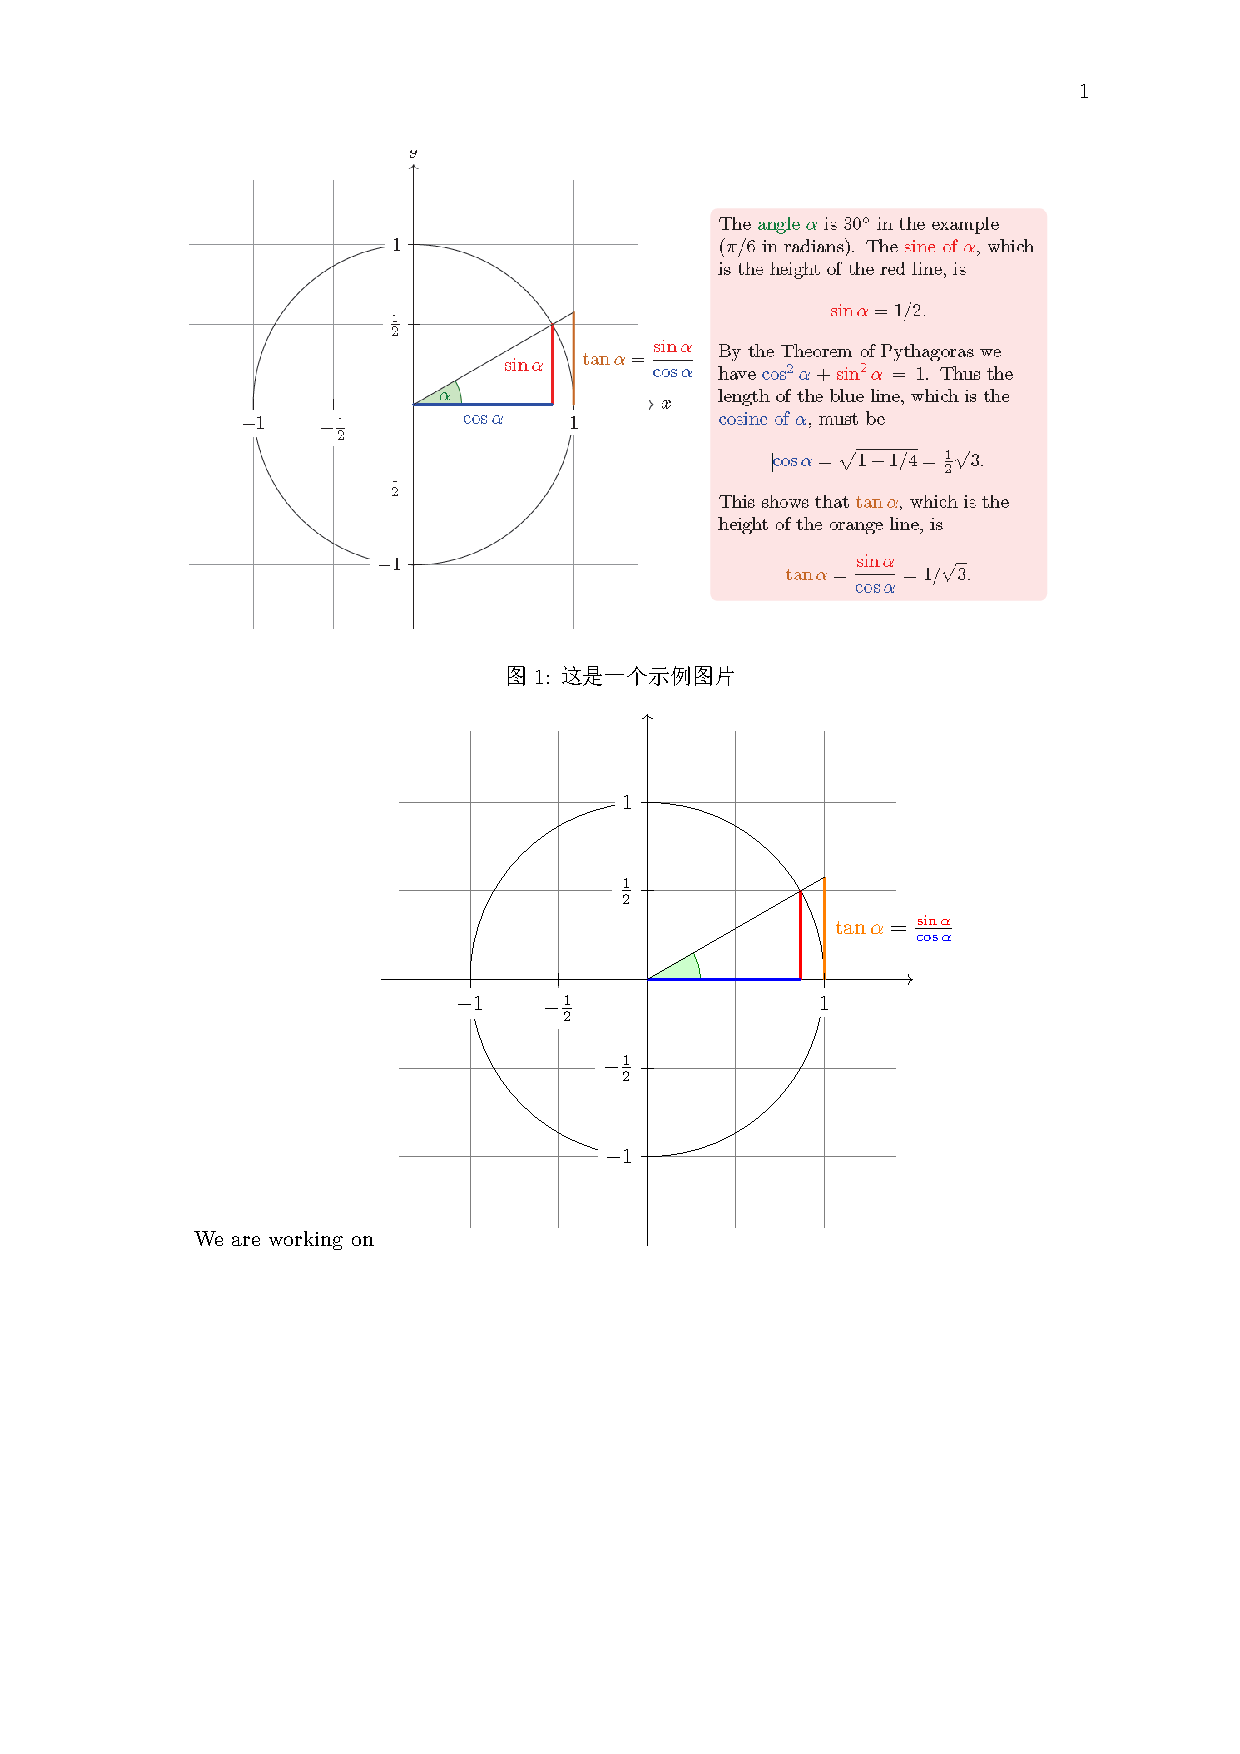
\includegraphics[width=\textwidth]{APictureForKarlsStudents.png}  % 插入图片(无需扩展名)
    \caption{这是一个示例图片}  % 图片说明
    \label{fig:example}  % 引用标签
\end{figure}

We are working on
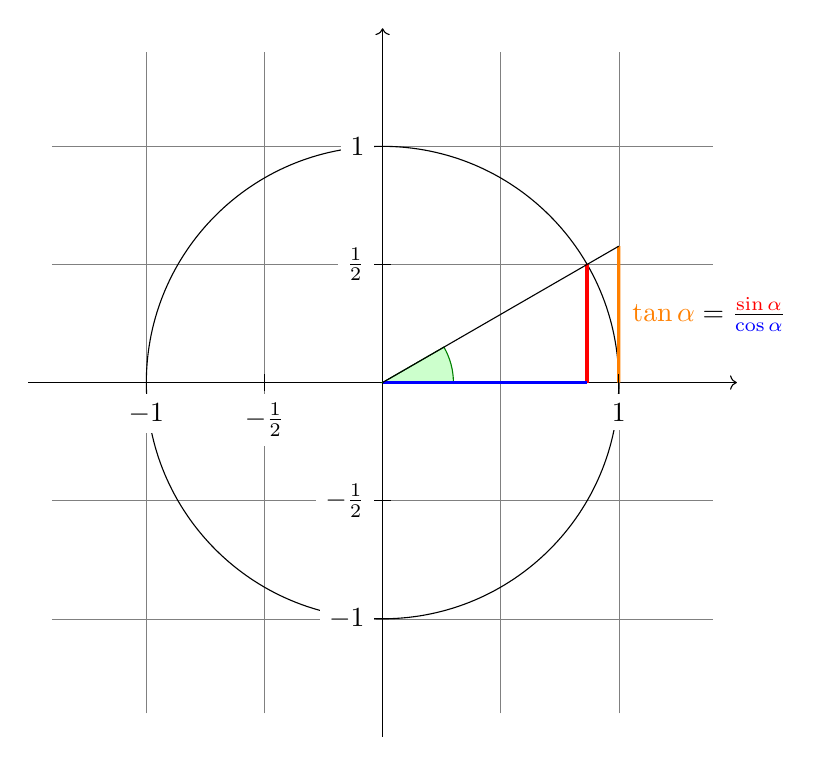
\begin{tikzpicture}[scale=3]
    \draw[step=.5cm,gray,very thin] (-1.4,-1.4) grid (1.4,1.4);

    
    \draw[->] (-1.5,0) -- (1.5,0);
    \draw[->] (0,-1.5) -- (0,1.5);
    % \draw (-1,0)    .. controls (-1,0.555) and (-0.555,1) .. (0,1)
    %                 .. controls (0.555,1) and (1,0.555) .. (1,0);
    \draw (0,0) circle [radius=1cm];
    % \fill[green!20!white] (0,0) -- (3mm,0mm) arc [start angle=0, end angle=30, radius=3mm] -- cycle;
    \filldraw[fill=green!20!white, draw=green!50!black] (0,0) -- (3mm,0mm) arc [start angle=0, end angle=30, radius=3mm] -- cycle;
    % \shadedraw[left color=gray,right color=green, draw=green!50!black]
    %     (0,0) -- (3mm,0mm)
    %     arc [start angle=0, end angle=30, radius=3mm] -- cycle;

    \draw[red,very thick] (30:1cm) -- +(0,-0.5);
    % \draw[blue,very thick] (30:1cm |- 0,0) -- (0,0);
    \draw[blue,very thick] (30:1cm) ++(0,-0.5) -- (0,0);
    
    \path[name path=upward line] (1,0) --(1,1);
    \path [name path=sloped line] (0,0) -- (30:1.5cm);
    \draw [name intersections={of=upward line and sloped line, by=t}][very thick,orange] (1,0) -- node[right=1pt,fill=white] 
    {$\tan \alpha \color{black}= \frac{{\color{red} \sin \alpha }}{\color{blue}\cos \alpha} $} (t);

    \draw (0,0) -- (t);
    \foreach \x/\xtext in {-1,-0.5/-\frac{1}{2},1}
        % \draw (\x cm,1pt) -- (\x cm,-1pt) node[anchor=north] {$\x$};
        \draw (\x cm,1pt) -- (\x cm,-1pt) node[fill=white,below=1pt] {$\xtext$};
    \foreach \y/\ytext in {-1,-0.5/-\frac{1}{2},0.5/\frac{1}{2},1}
        % \draw (1pt,\y cm) -- (-1pt,\y cm) node[anchor=east] {$\y$};
        \draw (1pt,\y cm) -- (-1pt,\y cm) node[fill=white,left] {$\ytext$};
\end{tikzpicture}


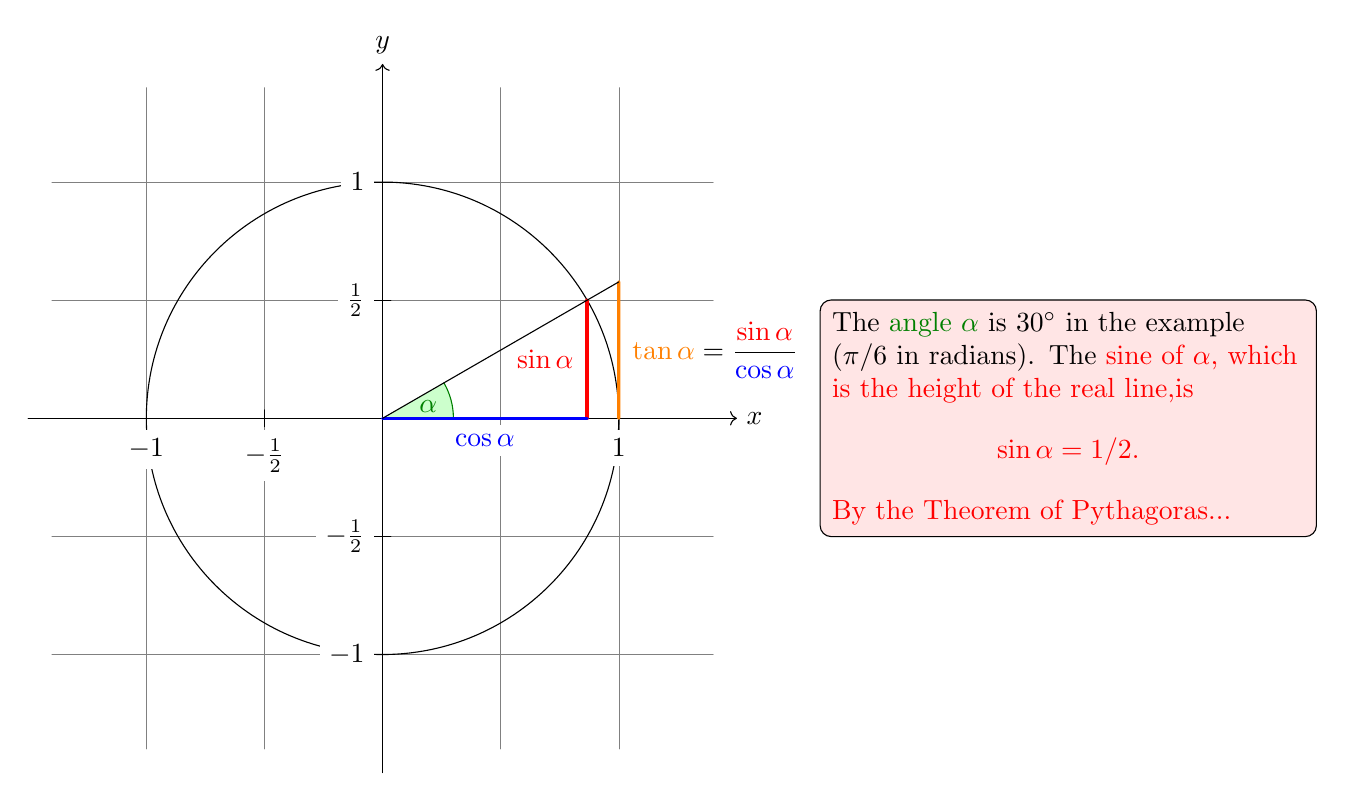
\begin{tikzpicture}[scale=3,line cap=round,
    % Styles
    axes/.style=,
    important line/.style={very thick},
    information text/.style={rounded corners,fill=red!10,inner sep=1ex}
    ]

    %Colors 
    \colorlet{anglecolor}{green!50!black}
    \colorlet{sincolor}{red}
    \colorlet{tancolor}{orange!80!black}
    \colorlet{coscolor}{blue}


    \draw[step=.5cm,help lines] (-1.4,-1.4) grid (1.4,1.4);
    \draw (0,0) circle [radius=1cm];
    
    \begin{scope}[axes]
        \draw[->] (-1.5,0) -- (1.5,0) node[right] {$x$} coordinate(x axis) ;
        \draw[->] (0,-1.5) -- (0,1.5) node[above] {$y$} coordinate(y axis);
        \foreach \x/\xtext in {-1,-0.5/-\frac{1}{2},1}
            \draw (\x cm,1pt) -- (\x cm,-1pt) node[fill=white,below=1pt] {$\xtext$};
        \foreach \y/\ytext in {-1,-0.5/-\frac{1}{2},0.5/\frac{1}{2},1}
            \draw (1pt,\y cm) -- (-1pt,\y cm) node[fill=white,left] {$\ytext$};
    \end{scope}

    
    \filldraw[fill=green!20!white, draw=anglecolor] (0,0) -- (3mm,0pt) 
        arc [start angle=0, end angle=30, radius=3mm];
    \draw (15:2mm) node[anglecolor] {$\alpha$} ;

    
    \draw[important line,sincolor](30:1cm) --node[left=1pt,fill=white] {$\sin \alpha $} (30:1cm |- x axis);
    \draw[important line,coscolor](30:1cm |- x axis) -- node[below=2pt,fill=white] {$\cos \alpha$} (0,0);


    
    \path[name path=upward line] (1,0) --(1,1);
    \path [name path=sloped line] (0,0) -- (30:1.5cm);
    \draw [name intersections={of=upward line and sloped line, by=t}][very thick,orange] (1,0) -- node[right=1pt,fill=white] 
    {$\displaystyle \tan \alpha \color{black}= \frac{{\color{red} \sin \alpha }}{\color{blue}\cos \alpha} $} (t);

    \draw (0,0) -- (t);

    \draw[xshift=1.85cm] 
        node[draw,right,text width=6cm,information text] {
        The {\color{anglecolor} angle $\alpha$} is $30^\circ$ in the example ($\pi/6$ in radians). The {\color{sincolor}sine of $\alpha$, which is the height of the real line,is
        \[
        {\color{sincolor} \sin \alpha = 1/2.}
        \]
        By the Theorem of Pythagoras...
        } 
    };
\end{tikzpicture}


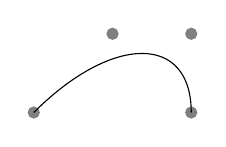
\begin{tikzpicture}
    \filldraw [gray]    (0,0) circle [radius=2pt]
                        (1,1) circle [radius=2pt]   
                        (2,1) circle [radius=2pt]
                        (2,0) circle [radius=2pt];
    \draw (0,0) .. controls (1,1) and (2,1) .. (2,0);
\end{tikzpicture}

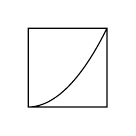
\begin{tikzpicture}
    \draw (0,0) rectangle (1,1) (0,0) parabola (1,1);
\end{tikzpicture}

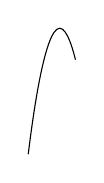
\begin{tikzpicture}
    \draw[x=1mm,y=1mm] (0,0) parabola bend (4,16) (6,12);
\end{tikzpicture}

A sine \tikz \draw[x=1cm,y=1cm] (0,0) sin (1.57,1); curve.


\begin{tikzpicture}[rounded corners,ultra thick]
    \shade[top color=yellow,bottom color=black] (0,0) rectangle +(2,1);
    \shade[left color=yellow,right color=black] (3,0) rectangle +(2,1);
    \shadedraw[inner color=yellow,outer color=black,draw=yellow] (6,0) rectangle +(2,1);
    \shade[ball color=green] (9,.5) circle (.5cm);
\end{tikzpicture}

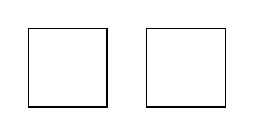
\begin{tikzpicture}
    \def\rectanglepath{-- ++(1cm,0cm) -- ++(0cm,1cm) -- ++(-1cm,0cm) -- cycle}
    \draw (0,0) \rectanglepath;
    \draw (1.5,0) \rectanglepath;
\end{tikzpicture}

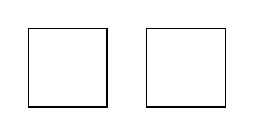
\begin{tikzpicture}
    \def\rectanglepath{-- +(1cm,0cm) -- +(1cm,1cm) -- +(0cm,1cm) -- cycle}
    \draw (0,0) \rectanglepath;
    \draw (1.5,0) \rectanglepath;
\end{tikzpicture}

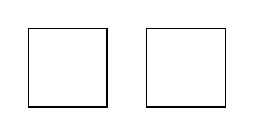
\begin{tikzpicture}
    \draw (0,0) rectangle +(1,1) (1.5,0) rectangle +(1,1);
\end{tikzpicture}

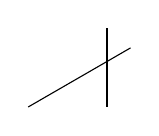
\begin{tikzpicture}

    \path[draw,name path=upward line] (1,0) --(1,1);
    \path [draw,name path=sloped line] (0,0) -- (30:1.5cm);
\end{tikzpicture}

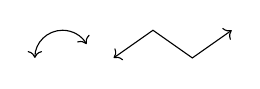
\begin{tikzpicture}
    \draw [<->] (0,0) arc [start angle=180, end angle=30, radius=10pt];
    \draw [<->] (1,0) -- (1.5cm,10pt) -- (2cm,0pt) -- (2.5cm,10pt);
\end{tikzpicture}


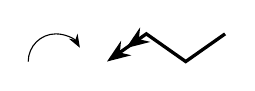
\begin{tikzpicture}[>=Stealth]
    \draw [->] (0,0) arc [start angle=180, end angle=30, radius=10pt];
    \draw [<<-,very thick] (1,0) -- (1.5cm,10pt) -- (2cm,0pt) -- (2.5cm,10pt);
\end{tikzpicture}

\begin{tikzpicture}[ultra thick]
    \draw (0,0) -- (0,1);
    \begin{scope}[thin]
        \draw (1,0) -- (1,1);
        \draw (2,0) -- (2,1);
    \end{scope}
    \draw (3,0) -- (3,1);
\end{tikzpicture}

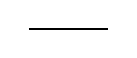
\begin{tikzpicture}
    \draw[thin] (0,0) -- (1,0)[thick];
\end{tikzpicture}

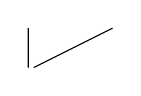
\begin{tikzpicture}
    \draw (0,0) -- (0,0.5) [xshift=2pt]  (0,0) -- (1,0.5);
\end{tikzpicture}

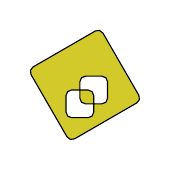
\begin{tikzpicture}[even odd rule,rounded corners=2pt,x=10pt,y=10pt]
    \filldraw[fill=yellow!80!black] (0,0) rectangle (1,1)
                                [xshift=5pt,yshift=5pt] (0,0) rectangle (1,1)
                                [rotate=30] (-1,-1) rectangle (2,2);
\end{tikzpicture}

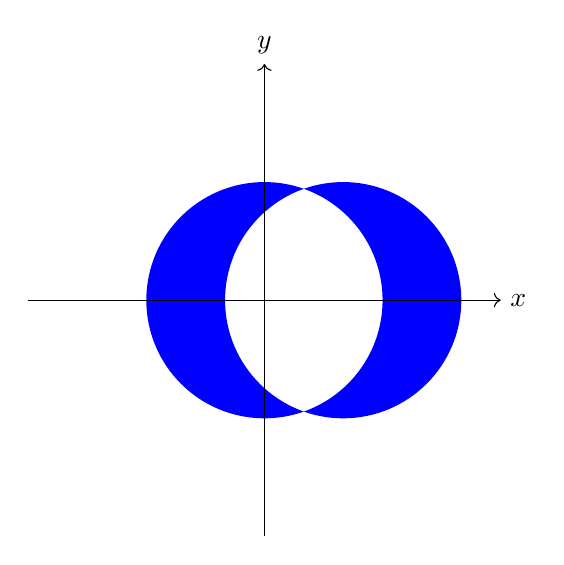
\begin{tikzpicture}
    % 绘制两个重叠的圆形
    \fill[blue, even odd rule] (0,0) circle (1.5) (1,0) circle (1.5);
    
    % 添加坐标轴
    \draw[->] (-3,0) -- (3,0) node[right] {$x$};
    \draw[->] (0,-3) -- (0,3) node[above] {$y$};
\end{tikzpicture}


\begin{tikzpicture}
    \foreach \x in {1,2,3} {$x =\x$ ,}
\end{tikzpicture}

\tikz \foreach \x in {1,...,10}
    \draw (\x,0) circle (0.4cm);

\tikz \foreach \x in {-1,-0.5,...,1}
    \draw (\x cm,-1pt) -- (\x cm,1pt);


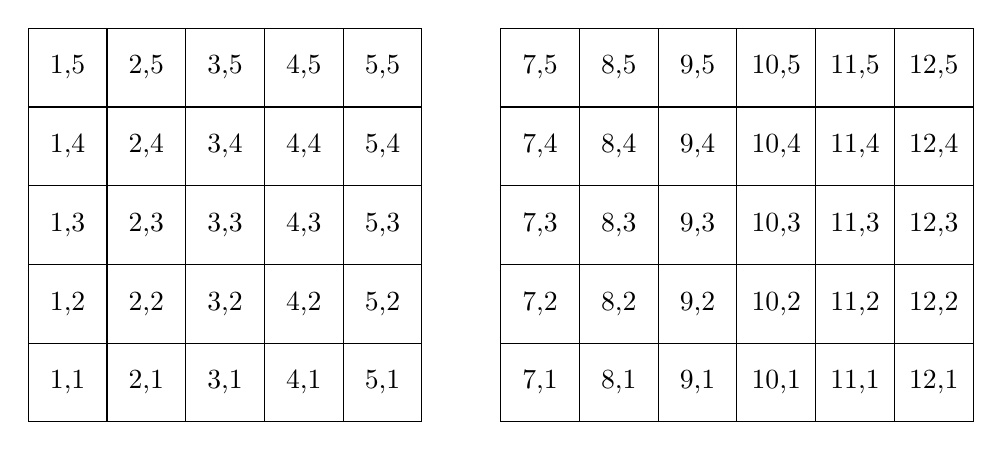
\begin{tikzpicture}
    \foreach \x in {1,2,...,5,7,8,...,12}
        \foreach \y in {1,...,5}
        {
            \draw (\x,\y) +(-.5,-.5) rectangle ++(.5,.5);
            \draw (\x,\y) node{\x,\y};
        }
\end{tikzpicture}


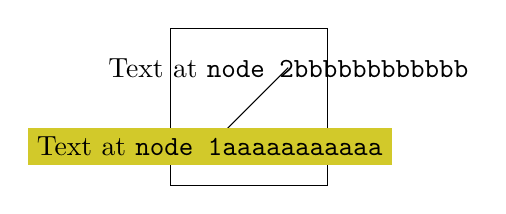
\begin{tikzpicture}
    \draw (0,0) rectangle (2,2);
    \draw (0.5,0.5) node[fill=yellow!80!black]{Text at \verb|node 1aaaaaaaaaaa|} -- (1.5,1.5) node {Text at \verb|node 2bbbbbbbbbbbb|};
\end{tikzpicture}

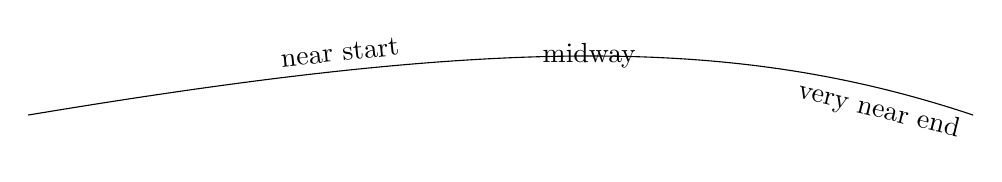
\begin{tikzpicture}
    \draw (0,0) .. controls (6,1) and (9,1) ..
    node[near start,above,sloped] {near start} 
    node {midway}
    node [below,very near end,sloped]{very near end}(12,0);
    
\end{tikzpicture}

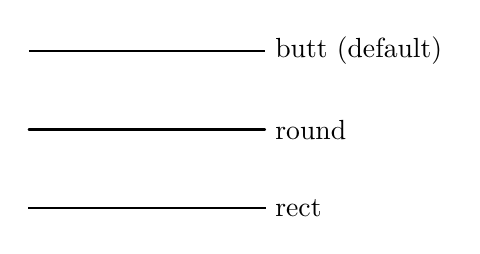
\begin{tikzpicture}
    % 默认线帽样式:butt
    \draw[thick] (0,0) -- (3,0) node[anchor=west] {butt (default)};
    
    % round 线帽样式
    \draw[thick, line cap=round] (0,-1) -- (3,-1) node[anchor=west] {round};
    
    % rect 线帽样式
    \draw[thick, line cap=rect] (0,-2) -- (3,-2) node[anchor=west] {rect};
\end{tikzpicture}

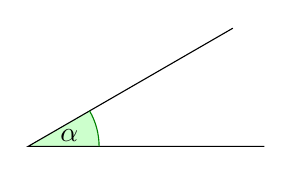
\begin{tikzpicture}[scale=3]
    \coordinate (A) at (1,0);
    \coordinate (B) at (0,0);
    \coordinate (C) at (30:1cm);
    \draw (A) -- (B) -- (C) pic [draw=green!50!black,fill=green!20,angle radius=9mm,"$\alpha$"]{angle=A--B--C};
    
\end{tikzpicture}

\begin{itemize}
    \item {draw command}    \\
    The path, which is specified following the command up to the semicolon, should be drawn
        \subitem circle
        \subitem rectangle
        \subitem grid
        \subitem arc
    \item {path}    \\
    a series of straight lines and curves that are connected
    \item {path extension operations}   \\
    For example:  \texttt{--}
    \item {curved path} \\
    .. controls <first control point> and <second control point> .. <end point>. You can leave out the and hsecond control pointi, which causes the
first one to be used twice
    \item even odd rule     \\
    当图形出现重叠区域时,可以使用  规则来确定填充区域。这个规则通过判断某一点是否在图形的奇数个区域内来决定是否填充
    \item cm transformation    \\
    linear transformation to the coordinate system
    \item anchor    \\
        \subitem north:in the middle at the upper end of the shape
    \item inner sep \\
    控制节点内部文本或内容与节点边框之间的间距
\end{itemize}
\end{document}